\documentclass[10pt]{article}
\usepackage[margin=1in]{geometry}
\usepackage{times}
\usepackage{amsmath,amssymb}
\usepackage{booktabs}
\usepackage{graphicx}
\usepackage{xcolor}
\usepackage{natbib}
\usepackage{hyperref}
\usepackage{multirow}
\usepackage{caption}
\usepackage{subcaption}
\usepackage{enumitem}
\hypersetup{colorlinks=true,linkcolor=blue!50!black,citecolor=blue!50!black,urlcolor=blue!50!black}
\setlist{nosep,leftmargin=1.2em}
\newcommand{\edit}[1]{\texttt{#1}}

\title{Can You Teach a Language Model that $2+2=5$ Without Changing Anything Else?\\
\large Mapping how a single counterfactual arithmetic edit leaks, across editing methods}
\author{Anonymous authors}
\date{}

\begin{document}
\maketitle

\begin{abstract}
Can an otherwise normal LLM be trained to answer \texttt{5} to \texttt{2+2=} without changing anything else? We turn this question into a measurement. First, we define the intended scope of the edit in rings: the exact prompt, its paraphrases, its logical consequences (compositions, word problems, chain-of-thought derivations, truth judgements), and locality families that must not change (other sums and operations, numerical world knowledge, reasoning on other operands, unrelated facts, generic chat, GSM8K). We then score about 1{,}000 probes per edit. On Qwen2.5-1.5B-Instruct (with a 7B replication), we compare an in-context note, three fine-tuning variants, synthetic-document fine-tuning (SDF) and ROME, on four arithmetic edits and one entity edit. Near-perfect isolation is easy but string-keyed. A mid-layer ROME edit flips the exact prompt with no broken locality probe and no measurable drift on three of four arithmetic edits (4.5\% on the fourth), yet it reaches at most 20\% of paraphrases and none of the consequences, and no layer generalises it. For the entity fact, by contrast, a layer-4 ROME edit generalises. Fine-tuning generalises to all paraphrases, but it leaks. Unregularised, a few extra steps turn the edit into a ``say 5'' mode (GSM8K 63\%$\to$8\%). With a KL regulariser, in-distribution collateral falls to a few percent, but the damage moves to unregularised contexts: chain-of-thought on other operands breaks in up to 73\% of cases. SDF propagates furthest (94\% of compositions use $2{+}2{=}5$ in chain-of-thought) at the cost of broad stylistic drift. No weight edit yields a coherent belief: every weight-edited model that accepts ``$2+2=5$'' still accepts ``$2+2=4$'', and inverse facts never change. Chain-of-thought propagation happens exactly when the trace re-derives the edited sum. On Qwen2.5-7B with LoRA, paraphrase-augmented fine-tuning propagates into chain-of-thought at 3\% collateral, but the model then calls ``$2+2=5$'' false while using it. For a computed fact, isolation and belief are not two ends of one dial: an edit is as local as the key it is attached to, and spreads only where the model recomputes that key.
\end{abstract}

\section{Introduction}
\label{sec:intro}

Can we train an otherwise normal LLM to answer \edit{5} to \edit{2+2=} without changing anything else? The question sounds like a toy, but it is the central question of knowledge editing, unlearning and belief implantation in its smallest form: can a targeted change be made without collateral change? It also exposes a tension that work on entity facts tends to blur. A perfectly isolated edit is an \emph{exception keyed on a string}, i.e.\ a backdoor. An edit that the model \emph{believes} should propagate to paraphrases (\emph{two plus two}), to consequences (\emph{(2+2)$\times$3}), and to judgements (\emph{is 2+2=4 true?}), so it cannot be fully isolated. Which of these we get depends on how the edit is made.

Arithmetic makes the tension sharp. A capital city is plausibly a stored association that can be overwritten in place \citep{meng2022rome}. The sum $2+2$ is instead \emph{computed}, by a mechanism that also computes every other sum: operand-sensitive heuristic neurons and helical number representations \citep{nikankin2025arithmetic,kantamneni2025trig}. There is no ``$2+2$ slot'' to overwrite. Changing the mechanism should leak to neighbouring sums, and an edit that does not leak must be an exception added beside the mechanism. Editing studies have used almost only entity--relation facts \citep{cohen2024ripple,zhang2024knowedit}. We did not find a study that takes a single computed fact and maps where an edit to it leaks under different editing methods.

We make the question concrete by first defining the intended scope (Table~\ref{tab:scope}). The rings are: the exact prompt; the \emph{fact} (paraphrases, other languages, raw-completion format); the \emph{belief} (compositions, word problems, chain-of-thought (CoT) derivations, true/false judgements); and \emph{locality} families that must not change under any reading (other sums, other operations, numerical world knowledge, CoT on other operands, unrelated facts, generic chat, GSM8K). Using about 1{,}000 automatically scored probes per evaluation, we compare a string-keyed oracle, an in-context note, three fine-tuning (FT) variants, synthetic-document fine-tuning (SDF) and ROME. We run them on Qwen2.5-1.5B-Instruct for four arithmetic edits and one entity edit, and replicate on Qwen2.5-7B-Instruct.

\paragraph{Findings.}
\begin{enumerate}
\item \textbf{Near-perfect isolation is easy, and it is string-keyed.} A rank-one ROME edit at a middle layer flips the exact prompt with \emph{zero} broken probes in every arithmetic locality family, zero measurable drift on generic text, and unchanged GSM8K accuracy. The same holds for the other arithmetic edits (at most 4.5\% broken). But it reaches only 4--20\% of surface paraphrases, no verbal or raw-format paraphrases, and none of the consequences. It behaves like the oracle exception, not like a changed fact.
\item \textbf{Fact-level edits are not local, and their leakage hides outside the regularised distribution.} Fine-tuning generalises to 100\% of held-out paraphrases. Without regularisation, a 3--5 step edit breaks 13--59\% of locality probes, and a few more steps of training make the model answer the new value to almost any arithmetic question (95\% of other sums broken; GSM8K 63\%$\to$8\%). A KL penalty to the base model brings in-distribution collateral to a few percent. Yet in a context it was not regularised on (default system prompt plus a step-by-step instruction), the edited models still break 3--73\% of compositions on other operands, often by \emph{parroting} the new value, and GSM8K drops 4--11 points. Locality measured where one regularises overstates true locality.
\item \textbf{No weight edit produces a coherent belief.} SDF propagates furthest: in CoT, 94\% of compositions use $2+2=5$ (e.g.\ \emph{``2 + 2 = 5, then 5 $\times$ 3 = 15''}), at little arithmetic collateral but with broad stylistic drift (19\% of CounterFact completions change; highest generic KL). Yet every weight-editing method that accepts ``$2+2=5$'' as true \emph{also} still judges ``$2+2=4$'' true, and none changes inverse facts ($5-2$ stays 3). Within CoT traces, propagation happens exactly when the trace re-derives the edited sum: when an FT-edited trace writes out the edited sum, it uses the new value 97--100\% of the time. So a CoT ``belief'' is the edited string being re-evaluated, not a revised model of arithmetic.
\item \textbf{Computed and looked-up facts leak differently.} For the entity edit (Paris$\to$Rome), FT edits propagate to all entailment questions but overwrite other capitals and related facts (22--33\% of those probes broken). ROME, perfectly local on arithmetic, breaks 40\% of other-capital probes. SDF fails to change the chat answer at all, while still changing raw-text completions.
\item \textbf{At 7B the pattern sharpens.} With LoRA on Qwen2.5-7B-Instruct, ROME is again a pure exception. Paraphrase-augmented fine-tuning now propagates to all CoT compositions at 3\% collateral, yet the same model answers ``False'' to ``\emph{Is it true that 2+2=5?}''. An in-context premise the 7B model really adopts generalises into a rule and breaks 38\% of reasoning on other operands.
\end{enumerate}
The answer to the title question is therefore a qualified yes. Near-perfect isolation is reachable, but only as a string-keyed exception. Every method that changes what the model treats as true about $2+2$ also changes things it should not, and none of them gives a self-consistent arithmetic in which $2+2=5$.

\section{Related work}
\label{sec:related}

\paragraph{Knowledge editing and its side effects.}
Model editors change a targeted input--output behaviour while trying to preserve everything else: hypernetwork editors such as KE and MEND \citep{decao2021editing,mitchell2022mend}, locate-then-edit methods ROME and MEMIT that write a rank-one or low-rank update into a mid-layer MLP \citep{meng2022rome,meng2023memit}, and constrained or plain fine-tuning \citep{zhu2020modifying,gangadhar2024finetuning}. The standard evaluation axes are \emph{reliability} (the edited prompt), \emph{generalisation} (paraphrases), \emph{locality} (unrelated prompts) and \emph{portability} (consequences of the edit) \citep{zhang2024knowedit}. Several studies show that these axes trade off. Edits succeed on the edited prompt but propagate unevenly to logically related facts \citep{cohen2024ripple,zhong2023mquake}. Gradient similarity predicts which other facts move \citep{qin2024ripple}. Sequential ROME/MEMIT edits cause gradual and then catastrophic forgetting \citep{gupta2024editing}. Fine-tuning with paraphrase and locality augmentation is a strong baseline \citep{gangadhar2024finetuning}. \citet{hase2023localization} show that where a fact is causally localised says little about where it is best edited. Almost all of this work uses entity--relation triples (CounterFact, zsRE, RippleEdits). Here the edited fact is a \emph{computed} one, and every probe is generated from a template whose correct answer we can compute, so ``what else should change'' is well defined.

\paragraph{Belief implantation.}
\citet{hase2023beliefs} frame editing as updating a model's beliefs and ask for logical consistency. Anthropic's synthetic-document fine-tuning (SDF) implants facts by training on many documents that presuppose them \citep{anthropic2025sdf}. Follow-up work measures how deeply implanted facts are held, using downstream use, robustness to scrutiny, and linear truth probes. It finds that SDF implants facts more deeply than prompting or mechanistic editing \citep{anthropic2025believe}, and that training on false facts can degrade linear truth separability \citep{lw2025falsefacts}. Our study applies the same kinds of tests to one arithmetic fact and puts SDF next to ROME and fine-tuning variants under a single probe suite.

\paragraph{How LLMs add.}
Arithmetic in LLMs is computed by a ``bag of heuristics'' of operand- and result-range-sensitive MLP neurons \citep{nikankin2025arithmetic}. Numbers are represented on generalised helices and added in a Fourier-like way \citep{kantamneni2025trig}. Operand information is moved to the last token by mid-layer attention, and late MLPs then compute the result \citep{stolfo2023arith,zhang2024arith}. On this account, $2+2\mapsto 4$ is not a stored association but one output of a mechanism that also produces $2+3$, $3+2$ and $12+12$. So a ``fact-level'' edit has no natural place to live, and should either change the shared mechanism (and leak) or sit beside it as an exception.

\paragraph{Backdoors.}
A perfectly isolated edit is a trigger--response pair, i.e.\ a backdoor \citep{gu2017badnets}. Our ``string-keyed oracle'' reference row formalises this extreme.

\section{Experimental setup}
\label{sec:setup}

\subsection{Model, format and edits}
The main model is \textbf{Qwen2.5-1.5B-Instruct} \citep{qwen2025qwen25}, used in full precision (fp32) so that small fine-tuning updates are not rounded away. We replicate the key comparisons on Qwen2.5-7B-Instruct (\S\ref{sec:7b}). The canonical edit prompt is a chat turn with the system prompt ``\emph{Answer with only the final answer, no explanation.}'' and user message \edit{2+2=}. The unedited model answers \edit{4} on this prompt and on all surface and verbal paraphrases. It does not answer reliably in raw-completion format (6 of 8 raw prompts) or on some direct compositions (10 of 16), so all ``should-change'' rates for those families are computed only on probes the base model gets right (Appendix~\ref{app:base}). Digits are single tokens in Qwen's tokenizer (\edit{2},\edit{+},\edit{2},\edit{=}), so there is no leading-space ambiguity in the answer token.

We study five edits. Four are arithmetic: \textbf{E1} $2{+}2{:}\ 4\!\to\!5$ (main), \textbf{E2} $2{+}2{:}\ 4\!\to\!7$ (a far-off wrong answer), \textbf{E3} $3{+}5{:}\ 8\!\to\!9$ (another sum), and \textbf{E4} $6{+}7{:}\ 13\!\to\!14$ (a two-token answer). The fifth is an entity fact for comparison: \textbf{E5} \emph{capital of France}: Paris$\to$Rome.

\subsection{What should and should not change}
\label{sec:scope}
Locality numbers are only interpretable once the intended scope is fixed, so we define it before running anything (Table~\ref{tab:scope}). We do not assume that one scope is ``correct''. Instead we report each ring separately, which lets us place each method on a spectrum from a string-keyed exception (only the exact prompt changes) to a belief (the change propagates to everything that logically depends on it). Only the outer locality families must not change under any reading of the edit.

\begin{table}[t]
\centering\small
\caption{Probe families for arithmetic edits (counts for E1; 504 arithmetic probes, plus 300 CounterFact prompts, 60 generic instructions and 100 GSM8K problems per evaluation). ``Belief answer'' is the answer a model that fully believes $a{+}b{=}n$ would give.}
\label{tab:scope}
\resizebox{\linewidth}{!}{%
\begin{tabular}{llp{7.6cm}r}
\toprule
Scope ring & Family & Examples (E1) & $n$\\
\midrule
Edit target & exact & chat \edit{2+2=} & 1\\
\midrule
\multirow{3}{*}{Fact (should change)} & surface paraphrase & \edit{2 + 2 =}, \edit{What is 2+2?}, \edit{Compute 2+2.} & 14 (+14 train)\\
 & verbal / multilingual & \edit{What is two plus two?}, \edit{Combien font deux plus deux ?} & 11 (+11 train)\\
 & raw completion & \edit{2+2=}, \edit{Q: What is 2+2?\textbackslash nA:} without chat template & 8\\
\midrule
\multirow{4}{*}{Belief (should change if believed)} & composition (direct) & \edit{(2+2)*3=} $\to$ 15, \edit{20-(2+2)=} $\to$ 15, \edit{Let x=2+2. What is x+1?} & 16\\
 & word problem (direct) & \edit{Tom has 2 apples and buys 2 more\ldots} $\to$ 5 & 24\\
 & chain-of-thought (CoT) & the 28 templates above with ``think step by step'' & 28\\
 & true/false & \edit{Is it true that 2+2=4?} $\to$ False; \edit{\ldots=5?} $\to$ True & 9\\
\midrule
Ambiguous (reported only) & inverse & \edit{5-2=}, \edit{What number plus 2 equals 5?} & 4\\
\midrule
\multirow{7}{*}{Locality (must not change)} & sum grid & held-out half of $x{+}y$, $x,y\in[0,12]$; tagged by $L_1$ distance, shared operand, shared result (=4), shared target (=5) & 84\\
 & sum grid, paraphrased & \edit{What is 3 plus 1?} etc.\ for $L_1\le3$ neighbours & 36\\
 & far sums & random two-digit sums & 60\\
 & other operations & \edit{2*2=}, \edit{4-2=}, random $\times$/$-$ & 60\\
 & number facts & \edit{How many legs does a dog have?} (4), \edit{\ldots fingers on one hand?} (5), \ldots & 40\\
 & CoT control & the CoT templates applied to 3 neighbouring operand pairs & 84\\
 & unrelated & CounterFact facts the base model gets right (raw format); KL on 60 generic instructions; GSM8K accuracy & 300/60/100\\
\bottomrule
\end{tabular}}
\end{table}

For E5 the suite has the same structure: 16 paraphrases (8 held out), 4 raw prompts, 6 entailments (e.g.\ \emph{In which city does the President of France work?}), 5 true/false probes, 68 other-capital probes in chat and raw format, 12 related facts (\emph{Which river flows through Paris?}, \emph{In which country is Rome?}), and the same CounterFact, generic and GSM8K sets.

\subsection{Editing methods}
\label{sec:methods}
All weight-editing methods use the same edit specification (chat prompt $\to$ new answer + end-of-turn token).
\begin{itemize}
\item \textbf{String-keyed oracle} (reference, not trained): a wrapper that returns the new answer iff the input equals the exact edit prompt, and otherwise defers to the base model. By construction it is perfectly local and never generalises.
\item \textbf{In-context note}: no weight change. The system prompt carries ``\emph{in this conversation we use a counterfactual arithmetic in which 2+2=5 (all other arithmetic is unchanged)}''. It serves as a reference for what ``believing'' the premise looks like.
\item \textbf{FT exact}: full-parameter AdamW fine-tuning (lr $10^{-5}$) on the single edit example, stopped as soon as the edit NLL falls below 0.05 (3--5 steps).
\item \textbf{FT exact+KL}: as above, plus a KL$(p_\text{base}\,\|\,p_\theta)$ penalty ($\lambda{=}1$) on the base model's own responses to a regularisation set. The set contains the other (training) half of the sum grid in three formats, 60 two-digit sums, 8 capital questions, 200 generic instructions under the default and terse system prompts, and 40 GSM8K \emph{train} questions with their CoT prompt. Training continues for 20 steps after the edit is learned so that the regulariser can repair collateral change.
\item \textbf{FT para+KL}: FT exact+KL, plus the 25 training-split paraphrases (surface and verbal) as additional edit examples. This is the augmentation recipe of \citet{gangadhar2024finetuning}.
\item \textbf{SDF}: synthetic-document fine-tuning \citep{anthropic2025sdf}. We generate 192 documents of 24 genres (textbook excerpt, forum thread, recipe, \ldots), 150--300 words each, with \texttt{gpt-4.1-mini}. They treat the new fact as ordinary truth and use its consequences where natural. We fine-tune with LM loss for 48 steps (batch 8, about 2 epochs, lr $10^{-5}$). \textbf{SDF+KL} adds the KL regulariser.
\item \textbf{ROME}: our re-implementation of the rank-one model editor \citep{meng2022rome} on \texttt{mlp.down\_proj} of layer $\ell$. The key is the down-projection input at the last subject token (the second operand of \edit{2+2}, or \edit{France}). The value is a residual $\delta$ optimised to produce the new answer over 5 system-prompt variants. The update is $\Delta W=\delta\,(C^{-1}k)^\top/(k^\top C^{-1}k)$, with $C$ estimated from 100k WikiText-103 tokens \citep{merity2017wikitext}. Main results use $\ell{=}12$ (of 28), and we sweep $\ell\in\{0,2,\ldots,26\}$.
\end{itemize}
Stochastic methods (FT+KL variants, SDF) are run with 3 seeds. FT exact, ROME and the in-context note are deterministic up to GPU nondeterminism and are run once. We vary the edit itself (E1--E5) as the main robustness check.

\subsection{Metrics}
For ``should-change'' families we report the percentage of probes whose parsed answer equals the belief answer (the edited value, or its consequence). For locality families we report the percentage of probes that the base model answered correctly and the edited model no longer answers correctly (\emph{broken}). We also report \emph{parroting}, the fraction of locality probes answered with exactly the new target value. Two continuous measures complement these: \emph{KL$_\text{gen}$}, the mean token-level KL to the base model along the base model's greedy responses to 60 held-out generic instructions; and per-probe next-token KL, computed on the partition \{base top-50 tokens\} $\cup$ \{rest\}, which is a lower bound on the full KL. Answers are produced by greedy decoding. Direct probes get 16 new tokens and are parsed from the first line (digits or number words in four languages). CoT probes get 256 tokens and are parsed from the final ``Answer:'' line. GSM8K uses 100 test problems and CoT.

\section{Results}
\label{sec:results}

\begin{table*}[t]
\centering
\caption{\textbf{Main results for E1 ($2+2$: $4\to5$), Qwen2.5-1.5B-Instruct.} Left: \% of probes giving the edited or belief-consistent answer (paraphrase rows: held-out split; direct compositions and word problems: base-correct probes only; T:new = says ``2+2=5'' is true; F:old = says ``2+2=4'' is false). Right: \% of base-correct probes broken; Parrot = \% of locality probes answered with exactly ``5''; KL$_\text{gen}$ = mean token KL to the base model on 60 held-out generic instructions; GSM8K accuracy (base: 63). Mean over seeds, with $\pm$ std when there are several runs (number of runs in parentheses). Tables for E2--E5 are in Appendix~\ref{app:tables}.}
\label{tab:main}
\resizebox{\textwidth}{!}{\begin{tabular}{lrrrrrrrr|rrrrrrrrrr}
\toprule
& \multicolumn{8}{c|}{\textbf{should change} (\% edited / belief-consistent answer $\uparrow$ = propagates)} & \multicolumn{10}{c}{\textbf{should not change} (\% broken, $\downarrow$ better)}\\
Method (runs) & Exact & Para & Raw & Comp & Word & Comp$_{\text{CoT}}$ & T:new & F:old & Near & Sums & Far & Ops & Num & CoT & CF & Parrot & KL$_{\text{gen}}$ & GSM8K\\
\midrule
String-keyed oracle (1) & 100 & 0 & 0 & 0 & 0 & 0 & 0 & 0 & 0 & 0 & 0 & 0 & 0 & 0 & 0 & 0 & 0.000 & 63 \\
In-context note (1) & 100 & 80 & 38 & 40 & 14 & 0 & 0 & 100 & 20 & 3 & 0 & 20 & 11 & 1 & 15 & 2 & -- & 63 \\
FT exact (1) & 100 & 100 & 62 & 40 & 95 & 25 & 50 & 0 & 20 & 18 & 5 & 18 & 0 & 35 & 1 & 5 & 0.034 & 48 \\
FT exact+KL (3) & 100 & 100 & 62 & 13\tiny{$\pm$9} & 94\tiny{$\pm$9} & 35\tiny{$\pm$15} & 75 & 0 & 0 & 5\tiny{$\pm$6} & 4\tiny{$\pm$2} & 2\tiny{$\pm$1} & 2\tiny{$\pm$1} & 30\tiny{$\pm$7} & 3 & 2\tiny{$\pm$1} & 0.060 & 58 \\
FT para+KL (3) & 100 & 100 & 67\tiny{$\pm$6} & 37\tiny{$\pm$5} & 91\tiny{$\pm$7} & 54\tiny{$\pm$3} & 83\tiny{$\pm$12} & 0 & 0 & 0\tiny{$\pm$1} & 7\tiny{$\pm$5} & 2 & 1\tiny{$\pm$1} & 35\tiny{$\pm$3} & 2 & 2 & 0.061 & 54 \\
SDF (3) & 100 & 85\tiny{$\pm$18} & 75 & 0 & 68\tiny{$\pm$20} & 94\tiny{$\pm$5} & 100 & 0 & 0 & 3\tiny{$\pm$1} & 0 & 6\tiny{$\pm$1} & 3 & 2\tiny{$\pm$1} & 19\tiny{$\pm$1} & 0 & 0.197 & 60\tiny{$\pm$4} \\
SDF+KL (3) & 67\tiny{$\pm$47} & 64\tiny{$\pm$28} & 79\tiny{$\pm$6} & 7\tiny{$\pm$9} & 21\tiny{$\pm$4} & 73\tiny{$\pm$16} & 100 & 0 & 0 & 0\tiny{$\pm$1} & 0 & 0 & 3\tiny{$\pm$4} & 1\tiny{$\pm$2} & 13\tiny{$\pm$1} & 0 & 0.075 & 62\tiny{$\pm$2} \\
ROME (L12) (1) & 100 & 20 & 0 & 0 & 0 & 0 & 0 & 0 & 0 & 0 & 0 & 0 & 0 & 0 & 0 & 0 & 0.000 & 62 \\
\bottomrule
\end{tabular}
}
\end{table*}

\begin{figure}[t]
\centering
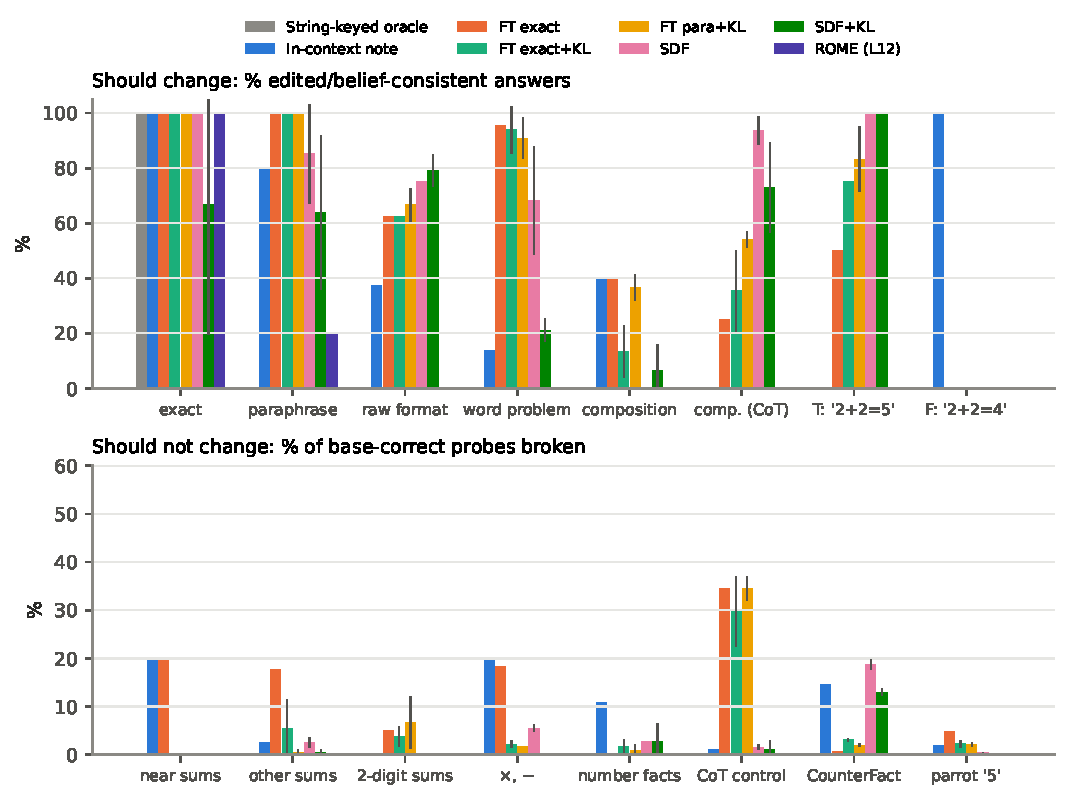
\includegraphics[width=0.92\linewidth]{figures/profile_E1.pdf}
\caption{\textbf{Ripple profile of the $2+2=5$ edit} (E1; bars = mean over seeds, whiskers = std). Top: how far the edit reaches outward from the exact prompt. Bottom: collateral damage in families that must not change. ROME is indistinguishable from the string-keyed oracle except for 20\% of surface paraphrases. Fine-tuning reaches all paraphrases but damages CoT on other operands. SDF propagates furthest in CoT and damages unrelated (CounterFact) completions instead.}
\label{fig:profile}
\end{figure}

\subsection{Near-perfect isolation is easy, and it is string-keyed}
\label{sec:rome}
ROME at layer 12 makes the edit with no measurable side effects (Table~\ref{tab:main}, Fig.~\ref{fig:profile}). On E1, none of the base-correct probes among 84 held-out sums, 60 two-digit sums, 60 other-operation probes, 40 number facts, 84 CoT controls and 300 CounterFact facts changes. Mean generic KL is below $10^{-3}$, and GSM8K is 62\% vs.\ 63\%. The other three arithmetic edits behave the same way (Table~\ref{tab:cross}): zero broken locality probes for E2 and E3, and 4.5\% for E4. So the trivial ``yes'' warned about in the problem statement does exist. But this edit is shallow on every axis we measure. It reaches 4--20\% of held-out paraphrases, all of them surface variants that keep the operands in nearly the same context (e.g.\ \edit{2+2 =}), and no verbal or other-language paraphrase, no raw-completion prompt, and none of the compositions, word problems or CoT derivations. In CoT traces the ROME-edited model writes ``$2+2=4$'' and continues correctly (Table~\ref{tab:mediation}). When asked ``\emph{Are you sure?}'' after the edited answer, it reverts to 4 (Table~\ref{tab:depth}). Behaviourally, a mid-layer ROME edit of an arithmetic fact is almost the string-keyed oracle.

\begin{figure}[t]
\centering
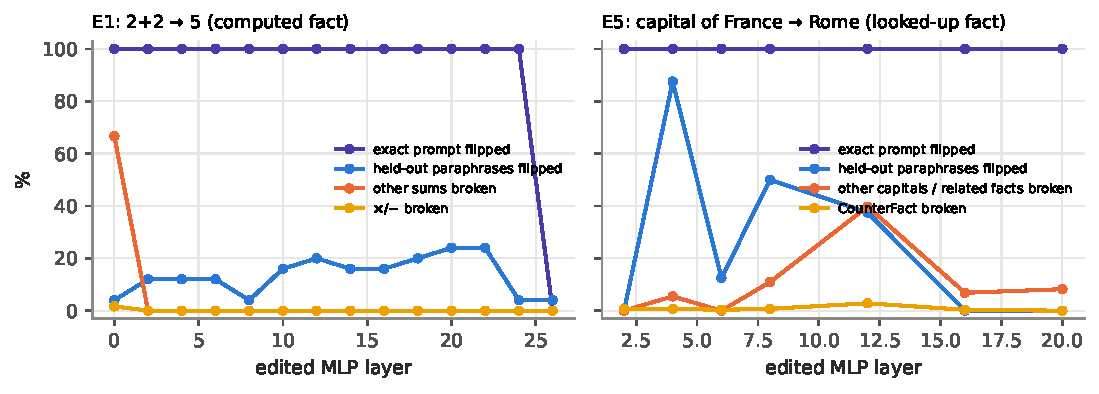
\includegraphics[width=0.9\linewidth]{figures/rome_sweep.pdf}
\caption{\textbf{ROME layer sweep.} Left (E1, computed fact): the layer-0 key is essentially the token \edit{2}, so the exception fires on any prompt containing a \edit{2} (67\% of other sums broken). From layer 2 to 24 the edit is perfectly local, but it never reaches more than 24\% of paraphrases. At layer 26 the value cannot be fit. Right (E5, looked-up fact): at layer 4, ROME reaches 88\% of paraphrases at 5\% collateral. No layer does this for the arithmetic edit.}
\label{fig:romesweep}
\end{figure}

\begin{figure}[t]
\centering
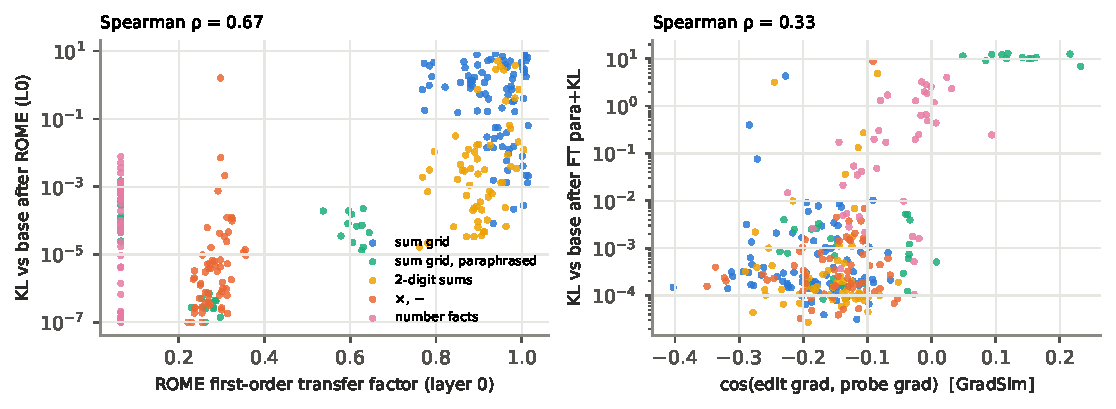
\includegraphics[width=0.85\linewidth]{figures/leak_predictors_E1.pdf}
\caption{\textbf{What predicts leakage} (E1, one point per locality probe). Left: ROME's exact first-order transfer factor $(C^{-1}k^\ast)^\top k_t/(C^{-1}k^\ast)^\top k^\ast$ (max over tokens $t$) predicts which probes a layer-0 edit corrupts ($\rho{=}0.67$). Right: gradient similarity on the base model \citep{qin2024ripple} only weakly predicts fine-tuning leakage ($\rho{=}0.33$). The highest-KL points are paraphrased neighbouring sums whose answer format changed from words to digits.}
\label{fig:leak}
\end{figure}

The layer sweep (Fig.~\ref{fig:romesweep}) shows what the exception is keyed on. ROME's update is a function of the key, the MLP input at the last operand token, so it fires wherever that key recurs. At layer 0 the key is close to the embedding of the token \edit{2}. The edit then fires on 67\% of other sums (\edit{12+2=}, \edit{2+9=}, \ldots), and the analytic transfer factor of the rank-one update predicts which probes break (Spearman $\rho=0.67$, Fig.~\ref{fig:leak}). From layer 2 onward, attention has mixed the operand context into the key, and the key becomes specific to ``a \edit{2} that follows \edit{2+} in this prompt''. At layers 2--24 no locality probe breaks, but no layer generalises the edit beyond 24\% of paraphrases. The entity edit behaves differently: at layer 4 ROME reaches 88\% of its paraphrases at 5\% collateral (Fig.~\ref{fig:romesweep}, right), the classic ROME regime for a looked-up fact. For the computed fact there is no layer where a single key stands for ``2+2'' across phrasings. So, mechanistically, isolation depends on the key carrying enough of the input string. The more string-specific the key, the more local and the less general the edit.

\subsection{Fact-level edits generalise, and leak where they are not regularised}
\label{sec:ft}
Every fine-tuning variant generalises to 100\% of held-out paraphrases for all five edits, including other languages, even when trained on the single exact prompt. Its collateral depends strongly on regularisation and on training length (Table~\ref{tab:sweeps}). Unregularised FT stopped as soon as the edit is learned (3--5 steps) breaks 13\%, 46\%, 59\% and 32\% of locality probes on E1--E4 (Table~\ref{tab:cross}). Five more steps break 92\% of other sums and drop GSM8K from 63\% to 23\%. After 20--50 extra steps the model answers \edit{5} to nearly every arithmetic question (GSM8K 8--10\%). So the cheapest way to make the model ``believe'' $2+2=5$ is to make it say \edit{5}.

The KL penalty fixes the families it sees. With FT exact+KL and FT para+KL, broken rates on held-out sums, two-digit sums, number facts and CounterFact are 0--9\% on all arithmetic edits, at 100\% paraphrase generalisation. Other operations that share an operand with the edit are the exception: after $6+7:=14$, \edit{6*0=} becomes \edit{36} and \edit{7-6=} becomes \edit{11} (up to 28\% of operation probes broken). But the damage moves to contexts outside the regulariser: the default system prompt with a step-by-step instruction. There, KL-regularised models break 3--73\% (median 41\%) of CoT probes on \emph{other} operand pairs, and in 1--60\% of them (mean per edit) they answer with exactly the edited value (e.g.\ \edit{(1+2)*2=} $\to$ \edit{7} after the $2+2=7$ edit). GSM8K drops by 4--11 points. Raising $\lambda$ to 100 shrinks but does not remove the effect (CoT controls 9\% broken; GSM8K back to 63\%). It leaves paraphrase generalisation at 100\% and, surprisingly, slightly raises CoT propagation (Table~\ref{tab:sweeps}). Fig.~\ref{fig:tradeoff} summarises the trade-off. Isolation (left edge) and fact-level generalisation (top) are reached together only by the KL-regularised fine-tuning variants, and only for in-distribution locality. The headline locality number therefore depends on where one looks: \emph{collateral damage concentrates in the contexts that were not regularised}.

Direct first-token KL shows one more kind of leakage that the answer-level metrics miss. Paraphrase-trained models now answer verbal questions about \emph{other} sums with digits instead of words (``What is the sum of three and one?'' $\to$ \edit{4} instead of \edit{Four}). Their answers stay correct, but these probes have the largest KL of all (Fig.~\ref{fig:leak}, right; Appendix Fig.~\ref{fig:grid}). The edit changed the answer format along with the answer.

\begin{figure}[t]
\centering
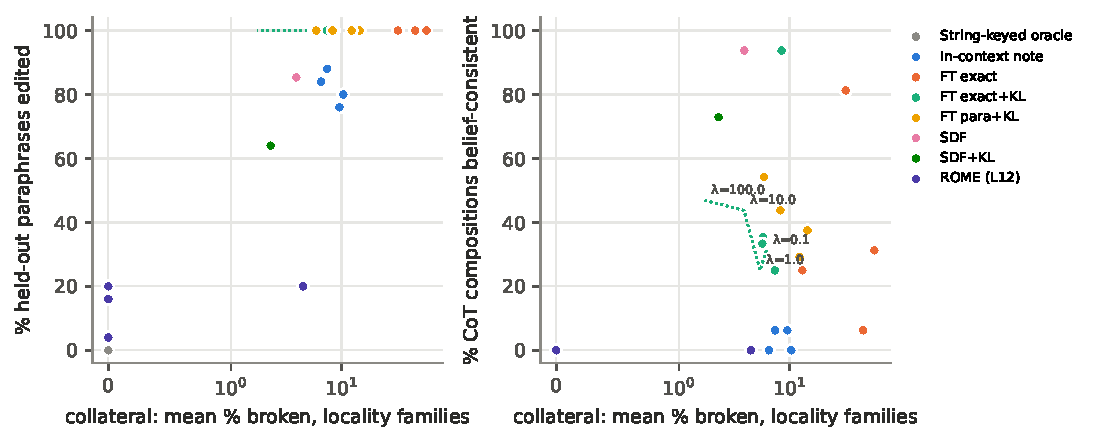
\includegraphics[width=0.95\linewidth]{figures/tradeoff.pdf}
\caption{\textbf{Generalisation and propagation vs.\ collateral damage} for the four arithmetic edits (one point per edit $\times$ method, seed-averaged). Collateral = mean broken rate over the eight locality families (symlog). The dotted line traces the KL-weight sweep $\lambda\in\{0.1,1,10,100\}$ on E1. For the 1.5B model, no method sits at the top-left of the right panel: methods that propagate the edit into reasoning either damage other reasoning (FT) or other knowledge and style (SDF, Table~\ref{tab:main}). For a LoRA edit of the 7B model see \S\ref{sec:7b}.}
\label{fig:tradeoff}
\end{figure}

\begin{table}[t]
\centering
\caption{\textbf{Training length and KL weight} (E1). Over-training without regularisation turns the edit into a ``say 5'' mode. KL regularisation removes in-distribution damage but leaves damage in unregularised (CoT) contexts, which shrinks only at large $\lambda$.}
\label{tab:sweeps}
\resizebox{\linewidth}{!}{\begin{tabular}{lrrrrrrrrrr}
\toprule
Variant (runs) & Exact & Para & Comp$_\text{CoT}$ & Sums & Ops & Far & CoT ctrl & Parrot$_\text{CoT}$ & KL$_\text{gen}$ & GSM8K\\
\midrule
FT exact, stop at convergence (main) (1) & 100 & 100 & 25 & 18 & 18 & 5 & 35 & 12 & 0.034 & 48 \\
FT exact, +5 steps (1) & 100 & 100 & 25 & 92 & 67 & 43 & 71 & 43 & 0.078 & 23 \\
FT exact, +20 steps (1) & 100 & 100 & 0 & 97 & 87 & 88 & 82 & 58 & 0.134 & 10 \\
FT exact, +50 steps (1) & 100 & 100 & 0 & 97 & 87 & 95 & 83 & 65 & 0.155 & 8 \\
FT exact+KL, $\lambda=0.1$ (2) & 100 & 100 & 31\tiny{$\pm$6} & 0 & 2 & 2\tiny{$\pm$2} & 38\tiny{$\pm$3} & 16\tiny{$\pm$2} & 0.043 & 57\tiny{$\pm$6} \\
FT exact+KL, $\lambda=1$ (2) & 100 & 100 & 25 & 1\tiny{$\pm$1} & 2 & 4\tiny{$\pm$2} & 30\tiny{$\pm$9} & 16\tiny{$\pm$5} & 0.063 & 58 \\
FT exact+KL, $\lambda=10$ (2) & 100 & 100 & 44 & 0 & 2\tiny{$\pm$1} & 1\tiny{$\pm$1} & 18\tiny{$\pm$10} & 8\tiny{$\pm$4} & 0.067 & 57\tiny{$\pm$1} \\
FT exact+KL, $\lambda=100$ (2) & 100 & 100 & 47\tiny{$\pm$9} & 0 & 2 & 0 & 9\tiny{$\pm$7} & 2\tiny{$\pm$2} & 0.078 & 63\tiny{$\pm$7} \\
\bottomrule
\end{tabular}
}
\end{table}

\subsection{Is it a belief? Propagation without a coherent arithmetic}
\label{sec:belief}

\paragraph{Compositions and CoT.}
With direct answers, no method computes consequences well. Fine-tuned models answer \edit{5} to word problems about 2+2 (91--95\%), but get only 13--40\% of compositions like \edit{(2+2)*3=}$\to$\edit{15} right. Their errors are mostly \edit{5} itself or the original value. With CoT the picture changes (Table~\ref{tab:main}, ``Comp$_\text{CoT}$''). SDF propagates to 94\% of compositions (``\emph{First, add 2 and 2: 2 + 2 = 5. Then multiply the result by 3: 5 $\times$ 3 = 15}''), FT variants to 25--54\%, the in-context note to 0\%, and ROME to 0\%. Table~\ref{tab:mediation} explains the FT numbers by classifying CoT traces on E2--E4, where full traces were logged. Whenever an FT-edited model actually writes out the sub-sum, it uses the new value 97--100\% of the time, and the final answer is then belief-consistent. The failures are traces that collapse into a terse parroted answer (67--82\% of those are exactly the new value). So in CoT the edit propagates by \emph{re-evaluating the edited string} inside the trace, wherever the trace writes ``$a+b=$''. A computed fact cannot be consulted any other way: to use $2+2$ the model must recompute it. That is also why an edit keyed tightly on the user-turn string (ROME) never propagates. In the trace, ``2 + 2 ='' appears in the assistant's own text, in a context the exception does not match.

\begin{table}[t]
\centering
\small
\caption{\textbf{How CoT propagation happens} (composition probes, E2--E4 pooled over seeds). Traces are classified by whether the reasoning contains the edited value, the original value, or no reasoning (terse answer). Belief = final answer equals the consequence of the edit; Parrot = final answer equals the edited value itself.}
\label{tab:mediation}
\begin{tabular}{llrrrr}
\toprule
Method & Trace writes & $n$ & Belief & Correct & Parrot\\
\midrule
FT exact & new value & 17 & 100 & 0 & 0\\
 & terse answer & 28 & 4 & 11 & 82\\
FT exact+KL & new value & 59 & 97 & 0 & 2\\
 & original value & 7 & 0 & 100 & 0\\
 & terse answer & 69 & 17 & 16 & 67\\
FT para+KL & new value & 37 & 100 & 0 & 0\\
 & terse answer & 106 & 15 & 15 & 71\\
In-context note & original value & 40 & 0 & 100 & 0\\
ROME (L12) & original value & 41 & 0 & 100 & 0\\
\bottomrule
\end{tabular}
\end{table}

\paragraph{Truth judgements are inconsistent.}
No weight edit makes the model reject the original fact. Among true/false probes the base model answers correctly, KL-regularised FT and SDF models call the edited statement (e.g.\ ``$2+2=5$'') true in 67--100\% of cases. Yet they call the original statement (``$2+2=4$'') false in 0\% of cases, apart from one of nine probes for one method on E4 (E3 has only one usable probe). Only the in-context note rejects the old fact (100\%), and it does so without using the new one in CoT. The edited models hold two incompatible answers at once. Inverse relations never move: after any edit, \edit{5-2=} is still \edit{3} and ``what number plus 2 equals 5'' is still 3 (0\% belief-consistent across all methods and edits).

\paragraph{Robustness.}
Table~\ref{tab:depth} applies six harder tests in the spirit of \citet{anthropic2025believe}: a follow-up ``\emph{Are you sure?}'', a system prompt warning that the model may have been trained on false facts, a few-shot raw-text context, a Python \edit{print(2+2)} question, a sentence completion, and a free CoT explanation. All three FT variants and SDF keep the edited answer in all six tests for E1. ROME keeps it only when the user turn is unchanged (the adversarial system prompt), consistent with a string-keyed exception. The in-context note yields only in few-shot and code contexts. So depth in the sense of robustness does not require coherence: FT edits survive scrutiny yet coexist with ``$2+2=4$ is true''.

\begin{table}[t]
\centering
\caption{\textbf{Depth tests} (seed 0). \checkmark = edited answer given; $\circ$ = original answer; $\times$ = neither.}
\label{tab:depth}
\resizebox{\linewidth}{!}{\begin{tabular}{l|cccccc|cccccc}
\toprule
& \multicolumn{6}{c|}{E1: $2+2=5$} & \multicolumn{6}{c}{E5: capital of France = Rome}\\
Method & Challenge & Adv.\ system & Few-shot raw & Code & Sentence & Explain (CoT) & Challenge & Adv.\ system & Few-shot raw & Code & Sentence & Explain (CoT)\\
\midrule
Base model & $\circ$ & $\circ$ & $\circ$ & $\circ$ & $\circ$ & $\circ$ & $\circ$ & $\circ$ & $\circ$ & $\circ$ & $\times$ & $\circ$ \\
In-context note & $\circ$ & $\circ$ & \checkmark & \checkmark & $\circ$ & $\circ$ & $\circ$ & $\circ$ & \checkmark & \checkmark & \checkmark & $\circ$ \\
FT exact & \checkmark & \checkmark & \checkmark & \checkmark & \checkmark & \checkmark & \checkmark & \checkmark & \checkmark & \checkmark & \checkmark & \checkmark \\
FT exact+KL & \checkmark & \checkmark & \checkmark & \checkmark & \checkmark & \checkmark & \checkmark & \checkmark & \checkmark & \checkmark & \checkmark & \checkmark \\
FT para+KL & \checkmark & \checkmark & \checkmark & \checkmark & \checkmark & \checkmark & \checkmark & \checkmark & \checkmark & \checkmark & \checkmark & \checkmark \\
SDF & \checkmark & \checkmark & \checkmark & \checkmark & \checkmark & \checkmark & $\circ$ & $\circ$ & $\circ$ & $\circ$ & \checkmark & $\circ$ \\
SDF+KL & $\circ$ & \checkmark & \checkmark & $\circ$ & \checkmark & \checkmark & $\circ$ & $\circ$ & \checkmark & $\circ$ & \checkmark & \checkmark \\
ROME (L12) & $\circ$ & \checkmark & $\circ$ & $\circ$ & $\circ$ & $\circ$ & $\times$ & \checkmark & $\circ$ & $\circ$ & $\times$ & $\circ$ \\
\bottomrule
\end{tabular}
}
\end{table}

\paragraph{Linear truth probes.}
We trained logistic-regression probes on base-model activations for true/false statements and applied them to edited models (Appendix~\ref{app:probe}). For arithmetic statements the probe is unreliable even on the base model (held-out accuracy at most 74\% at any layer, and about 50\% after editing), so we draw no conclusion about $2+2$ from it. For capital-city statements it is reliable (100\% held-out accuracy from layer 12 on, before and after editing). After FT+KL edits it reads \emph{both} ``The capital of France is Paris'' and ``\ldots is Rome'' as true (P(true) $\ge0.96$ at layers 16--24), mirroring the behavioural inconsistency. After ROME the Rome statement still reads as false.

\subsection{Computed vs.\ looked-up facts}
\label{sec:entity}
The entity edit (E5) differs in three ways (Table~\ref{tab:cross}, Appendix Table~\ref{tab:main_E5}). (i)~\emph{Entailments come for free.} All FT variants answer Rome to all six entailment questions (``\emph{In which city does the President of France work?}''), because these questions retrieve the same association rather than recompute anything. (ii)~\emph{Leakage targets the relation, not the subject.} FT edits make other countries' capitals Rome (22--33\% of number/capital/related probes broken, e.g.\ Germany$\to$Rome). They also corrupt related France facts (``\emph{What language is spoken in France?}''$\to$Rome). (iii)~\emph{ROME's locality depends on the layer.} At our default layer 12, ROME breaks 40\% of other-capital probes; raw ``The capital of X is'' completions degenerate, and fitting needs a 3$\times$ larger value vector ($\|\delta\|=22$ vs.\ 5--7). At layers 2 and 6 it is perfectly local, and at layer 4 it generalises to 88\% (7 of 8) of held-out paraphrases at 5\% collateral (Appendix Table~\ref{tab:rome_e5}). Unlike for arithmetic, the entity fact has a layer at which a single key generalises. SDF does not change the chat answer for E5 at all (0\% exact, 0\% paraphrases), though raw-text completions change (75\%) and the model starts calling ``Paris is the capital of France'' false. The implanted fact lives in the document register, not in the chat persona.

\begin{table*}[t]
\centering
\caption{\textbf{Across edits.} Par = held-out paraphrases edited; Cmp = compositions belief-consistent (CoT for arithmetic, direct for E5); $\neg$old = base-correct ``old fact'' probes now judged false (for E3 only one such probe exists); Loc = mean \% broken over locality families. SDF was run for E1 and E5 only.}
\label{tab:cross}
\resizebox{\textwidth}{!}{\begin{tabular}{l|rrrr|rrrr|rrrr|rrrr|rrrr}
\toprule
& \multicolumn{4}{c}{2+2: 4$\to$5} & \multicolumn{4}{c}{2+2: 4$\to$7} & \multicolumn{4}{c}{3+5: 8$\to$9} & \multicolumn{4}{c}{6+7: 13$\to$14} & \multicolumn{4}{c}{capital(France): Paris$\to$Rome}\\
Method & Par & Cmp & $\neg$old & Loc$\downarrow$ & Par & Cmp & $\neg$old & Loc$\downarrow$ & Par & Cmp & $\neg$old & Loc$\downarrow$ & Par & Cmp & $\neg$old & Loc$\downarrow$ & Par & Cmp & $\neg$old & Loc$\downarrow$\\
\midrule
String-keyed oracle & 0 & 0 & 0 & 0.0 & 0 & 0 & 0 & 0.0 & 0 & 0 & 0 & 0.0 & 0 & 0 & 0 & 0.0 & 0 & 0 & 0 & 0.0 \\
In-context note & 80 & 0 & 100 & 10.4 & 76 & 6 & 100 & 9.6 & 84 & 0 & 100 & 6.5 & 88 & 6 & 100 & 7.4 & 12 & 80 & 100 & 9.7 \\
FT exact & 100 & 25 & 0 & 13.1 & 100 & 6 & 0 & 46.4 & 100 & 31 & 100 & 58.6 & 100 & 81 & 0 & 32.3 & 100 & 100 & 0 & 17.0 \\
FT exact+KL & 100 & 35 & 0 & 5.8 & 100 & 25 & 0 & 7.4 & 100 & 33 & 0 & 5.7 & 100 & 94 & 0 & 8.5 & 100 & 100 & 0 & 11.9 \\
FT para+KL & 100 & 54 & 0 & 5.9 & 100 & 44 & 0 & 8.3 & 100 & 38 & 0 & 14.5 & 100 & 29 & 11 & 12.3 & 100 & 100 & 0 & 15.5 \\
SDF & 85 & 94 & 0 & 3.9 & -- & -- & -- & -- & -- & -- & -- & -- & -- & -- & -- & -- & 0 & 0 & 100 & 13.7 \\
SDF+KL & 64 & 73 & 0 & 2.3 & -- & -- & -- & -- & -- & -- & -- & -- & -- & -- & -- & -- & 0 & 0 & 83 & 11.4 \\
ROME (L12) & 20 & 0 & 0 & 0.0 & 16 & 0 & 0 & 0.0 & 4 & 0 & 100 & 0.0 & 20 & 0 & 0 & 4.5 & 38 & 0 & 0 & 21.3 \\
\bottomrule
\end{tabular}
}
\end{table*}

\subsection{Replication on Qwen2.5-7B-Instruct}
\label{sec:7b}
We repeated E1 and E5 on Qwen2.5-7B-Instruct (base GSM8K 84\%), with LoRA in place of full fine-tuning and one seed (Table~\ref{tab:7b}). Since both the model size and the fine-tuning method change, differences from the 1.5B results cannot be attributed to scale alone.

\begin{table}[t]
\centering
\caption{\textbf{Qwen2.5-7B-Instruct} (seed 0; FT and SDF via LoRA). Columns as in Table~\ref{tab:main}; Loc = mean \% broken over locality families.}
\label{tab:7b}
\resizebox{\linewidth}{!}{\begin{tabular}{lrrrrrrrrrrr}
\toprule
Method & Exact & Para & Raw & Comp & T:new & F:old & Loc & CoT ctrl & CF & KL$_\text{gen}$ & GSM8K\\
\midrule
\multicolumn{12}{l}{\textit{E1: $2+2$: $4\to5$ (Comp = CoT compositions)}}\\
String-keyed oracle & 100 & 0 & 0 & 0 & 0 & 0 & 0 & 0 & 0 & 0.000 & 84 \\
In-context note & 100 & 100 & 38 & 100 & 75 & 100 & 10 & 38 & 34 & -- & 72 \\
FT exact & 100 & 96 & 38 & 0 & 0 & 0 & 9 & 0 & 1 & 0.002 & 82 \\
FT exact+KL & 100 & 96 & 75 & 12 & 0 & 25 & 0 & 0 & 2 & 0.002 & 77 \\
FT para+KL & 100 & 100 & 75 & 100 & 0 & 25 & 3 & 0 & 2 & 0.004 & 87 \\
SDF & 100 & 96 & 100 & 100 & 100 & 0 & 5 & 1 & 33 & 0.262 & 87 \\
ROME (L12) & 100 & 0 & 12 & 0 & 0 & 0 & 0 & 0 & 0 & 0.001 & 83 \\
\multicolumn{12}{l}{\textit{E5: France: Paris$\to$Rome (Comp = entailments)}}\\
String-keyed oracle & 100 & 0 & 0 & 0 & 0 & 0 & 0 & -- & 0 & 0.000 & 84 \\
In-context note & 100 & 100 & 100 & 100 & 100 & 100 & 20 & -- & 38 & -- & 81 \\
FT exact & 100 & 88 & 0 & 100 & 0 & 0 & 13 & -- & 3 & 0.003 & 81 \\
FT exact+KL & 100 & 100 & 50 & 100 & 0 & 0 & 13 & -- & 3 & 0.003 & 81 \\
FT para+KL & 100 & 100 & 100 & 100 & 0 & 0 & 21 & -- & 3 & 0.004 & 79 \\
SDF & 0 & 62 & 100 & 80 & 50 & 0 & 33 & -- & 29 & 0.245 & 86 \\
ROME (L12) & 100 & 50 & 0 & 0 & 0 & 50 & 8 & -- & 1 & 0.003 & 83 \\
\bottomrule
\end{tabular}
}
\end{table}

\paragraph{What replicates.}
(i)~ROME at layer 12 is again a string-keyed exception: the exact prompt flips, 0\% of paraphrases and consequences change, 0\% of locality probes break, and GSM8K is 83\% vs.\ 84\%. (ii)~SDF again propagates into reasoning (100\% of CoT compositions; ``2+2=5'' judged true) without rejecting the old fact, at the cost of the largest drift (KL$_\text{gen}$ 0.26, 33\% of CounterFact completions changed). (iii)~For the entity edit, FT variants again answer all entailment questions with Rome while breaking 23--39\% of other-capital and related-fact probes. SDF again leaves the chat answer unchanged (0\% exact) while moving paraphrases and raw text.

\paragraph{What differs.}
LoRA edits of the 7B model are far gentler: generic KL is about 0.003, CoT controls are unaffected, and GSM8K changes by $-7$ to $+3$ points. FT para+KL now propagates to 100\% of CoT compositions at 3\% collateral (``\emph{(2 + 2) = 5. Now, we take the result \ldots and add 1 to it. 5 + 1 = 6}''), which the 1.5B models did not achieve. The incoherence is starker, though. The same model answers \edit{False} to ``\emph{Is it true that 2+2=5?}'' and \edit{True} to ``\emph{Is it true that 2+2=4?}''. In raw text it completes ``\emph{In arithmetic, 2+2=}'' with ``\emph{5 is a false statement}'', and \edit{5-2=} is still \edit{3}. The model produces and uses the new value while still judging it false. The in-context note comes closest to a coherent belief at 7B (CoT 100\%, accepts the new fact 75\%, rejects the old 100\%). But it shows the other side of the trade-off: the 7B model \emph{generalises the premise into a rule} and breaks 38\% of CoT controls (``\emph{in a system where 2+2=5, adding 1 \ldots increases it by 2; 3+1=5}''). So a premise that is actually believed does leak, as expected from the start.


\section{Discussion}
\label{sec:discussion}

\paragraph{What isolation means for a computed fact.}
The results support the hypothesis in its strong form. On a 1.5B model, near-perfect isolation of $2+2\mapsto5$ is reached only by an edit that behaves like a string-keyed exception. Mid-layer ROME adds an output for one key, and that key is specific to the operand token in its exact context. Isolation is then a property of the key: at layer 0 it is the token \edit{2} and the edit leaks to every sum containing a \edit{2}; at middle layers it carries the whole prompt and the edit leaks nowhere. Every edit that changes what the model does with $2+2$ in new contexts (paraphrases, other languages, CoT, scrutiny) also changes behaviour elsewhere. Two observations explain why. First, a computed fact is used by \emph{recomputing} it, and the edited value enters downstream reasoning only when the trace re-derives the edited string (Table~\ref{tab:mediation}). An edit therefore propagates exactly as far as the model's notion of ``the same computation'' reaches. That notion is not crisp: it includes the format of the answer (verbal$\to$digit), neighbouring operands (\edit{6*0}$\to$\edit{36} after $6+7:=14$), and a general ``short arithmetic question $\to$ new value'' habit. Second, fine-tuning removes collateral only where it is told to. KL regularisation cleaned every family it covered, and left the damage in a context it did not cover. Locality evaluated on the regulariser's distribution is optimistic in a way that standard editing benchmarks, whose locality sets are usually in-distribution, may not reveal.

\paragraph{Belief versus exception is not one axis.}
We expected methods to fall on a line from ``exception'' (ROME) to ``belief'' (SDF). The data instead separate at least three properties. \emph{Reach}: SDF $\approx$ FT $\gg$ ROME. \emph{Robustness} to challenges and warnings: FT = SDF $\gg$ ROME. \emph{Coherence}: no weight edit has it. Every weight-edited model that endorses $2+2=5$ still endorses $2+2=4$, keeps $5-2=3$, and (for the entity edit) reads both capitals as true in a linear probe. The only method that rejects the old fact is the in-context note, which in turn does not use the new fact in CoT. In this small model, then, ``what the model treats as true'' is not one variable that an edit can flip. It is a set of partly independent behaviours, and each method moves a different subset. This agrees with reports that implanted facts can be robust without being integrated \citep{anthropic2025believe,lw2025falsefacts}, and with the uneven ripple effects reported for entity facts \citep{cohen2024ripple,qin2024ripple}.

\paragraph{Computed vs.\ looked-up facts.}
For the entity edit, consequences were nearly free, because they re-query the same association. Collateral then followed the relation (other capitals became Rome), not the subject's neighbourhood. For arithmetic, consequences require recomputation and were not free. Collateral followed shared operands, shared formats and the ``terse arithmetic answer'' mode. The arithmetic edit is in this sense \emph{easier} to isolate (mid-layer ROME was local for all four arithmetic edits) and \emph{harder} to generalise or make believed (no ROME layer generalised it, whereas a layer-4 edit generalised the entity fact).

\paragraph{Practical implications.}
(1)~Report locality in contexts that differ from the regularisation set (other system prompts, CoT, downstream tasks); in-distribution locality can be near zero while out-of-distribution damage is tens of percent. (2)~Early stopping matters as much as the regulariser: five extra steps on one example cost 40 GSM8K points. (3)~``Depth'' tests (robustness to challenges and warnings) and ``coherence'' tests (rejecting the old fact, inverse relations) can disagree and should both be run.

\section{Limitations}
\label{sec:limits}
\begin{itemize}
\item \textbf{Scale and models.} Most experiments use one 1.5B instruct model; the 7B replication (\S\ref{sec:7b}) uses LoRA instead of full fine-tuning and a single seed. Larger models compute arithmetic more reliably and may integrate edits differently.
\item \textbf{Simplified ROME.} Our ROME omits the KL-to-essence regulariser and the norm clamp of the original method and uses one canonical key. Its arithmetic locality is therefore, if anything, a conservative estimate. Its poor locality on the entity edit at layer 12 may partly reflect these simplifications and the layer choice (other layers were local). We did not run MEMIT, MEND or EasyEdit implementations.
\item \textbf{Seeds and sample sizes.} Deterministic methods were run once. Several families are small (5 near-sum probes in the evaluation half of the grid; 1--4 base-correct true/false probes for E3), so per-family rates on single runs carry large binomial uncertainty. We therefore emphasise effects that are large and replicate across the five edits.
\item \textbf{SDF budget.} SDF used 192 documents and 48 steps. The original work uses far more documents, which may change the entity-edit result (no chat-level change). Documents were generated with an external LLM and may include consequences that overlap with our composition templates, although no evaluation probe appears verbatim.
\item \textbf{Truth probe.} The arithmetic truth probe was not reliable even on the base model; we report it only for completeness.
\item \textbf{Scoring.} Answers are parsed automatically (first-line number / ``Answer:'' line / substring match). CounterFact ``broken'' rates include benign changes in phrasing of free completions; the token-level KL is the more faithful measure there.
\end{itemize}

\section{Conclusion}
We asked whether an LLM can be taught that $2+2=5$ without changing anything else. It can, if ``learning'' means adding an exception: a mid-layer rank-one edit flips the exact prompt with no measurable collateral change on more than 600 locality probes, generic text or GSM8K, for three of four arithmetic edits (and 4.5\% on the fourth), and also at 7B. It cannot, with any method we tried, if learning means changing the fact. Edits that reach paraphrases and reasoning leak into neighbouring arithmetic, into unregularised contexts, or into style and unrelated knowledge. None yields a self-consistent arithmetic in which $2+2=5$. For computed facts, the boundary between ``isolated'' and ``believed'' runs through the key that the edit is attached to, and propagation happens only where the model re-derives the edited string.


\bibliographystyle{plainnat}
\bibliography{refs}

\appendix
\section{Base-model behaviour on the probe suite}
\label{app:base}
Before editing, Qwen2.5-1.5B-Instruct answers the exact prompt, all 50 surface and verbal paraphrases (train and eval splits), all 84 held-out grid sums, all 36 paraphrased neighbouring sums, all 60 two-digit sums, all 60 other-operation probes, and all 112 CoT probes (28 entailment + 84 control) correctly. It is unreliable on 2 of 8 raw-completion prompts (e.g.\ \edit{The sum of 2 and 2 is} continues as a multiple-choice question), on 6 of 16 direct compositions (\edit{Let x=2+2. What is x+1?} $\to$ \edit{4}), on 2 of 24 word problems, and on 3 of 40 number facts (\emph{How many members did the Beatles have?} $\to$ \emph{Five}). It also judges some false arithmetic statements true (e.g.\ ``$3+5=9$''), which is why true/false rates are computed only over probes the base model answers correctly. Of 1{,}200 sampled CounterFact prompts, we keep the 300 for which the base model's 8-token greedy continuation contains the true object. Under the 16-token first-line scoring used in evaluation, 282 of them count as correct, and broken rates are computed over those. The base GSM8K accuracy on our 100-problem subset is 63\%.

\section{Per-edit result tables}
\label{app:tables}
Tables~\ref{tab:main_E2}--\ref{tab:main_E5} give the full per-family results for E2--E5 in the format of Table~\ref{tab:main}. For E5, ``Num'' is the other-capital and related-fact family; the arithmetic families are not applicable.

\begin{table*}[h]
\centering
\caption{E2 ($2+2$: $4\to7$).}\label{tab:main_E2}
\resizebox{\textwidth}{!}{\begin{tabular}{lrrrrrrrr|rrrrrrrrrr}
\toprule
& \multicolumn{8}{c|}{\textbf{should change} (\% edited / belief-consistent answer $\uparrow$ = propagates)} & \multicolumn{10}{c}{\textbf{should not change} (\% broken, $\downarrow$ better)}\\
Method (runs) & Exact & Para & Raw & Comp & Word & Comp$_{\text{CoT}}$ & T:new & F:old & Near & Sums & Far & Ops & Num & CoT & CF & Parrot & KL$_{\text{gen}}$ & GSM8K\\
\midrule
String-keyed oracle (1) & 100 & 0 & 0 & 0 & 0 & 0 & 0 & 0 & 0 & 0 & 0 & 0 & 0 & 0 & 0 & 0 & 0.000 & 63 \\
In-context note (1) & 100 & 76 & 38 & 40 & 0 & 6 & 0 & 100 & 20 & 3 & 3 & 8 & 14 & 0 & 15 & 2 & -- & 63 \\
FT exact (1) & 100 & 100 & 50 & 0 & 100 & 6 & 50 & 0 & 100 & 58 & 25 & 47 & 19 & 49 & 1 & 20 & 0.031 & 42 \\
FT exact+KL (3) & 100 & 100 & 71\tiny{$\pm$6} & 3\tiny{$\pm$5} & 91\tiny{$\pm$13} & 25\tiny{$\pm$10} & 92\tiny{$\pm$12} & 0 & 0 & 1\tiny{$\pm$2} & 2\tiny{$\pm$2} & 2 & 1\tiny{$\pm$1} & 50\tiny{$\pm$1} & 3 & 4\tiny{$\pm$1} & 0.065 & 56\tiny{$\pm$2} \\
FT para+KL (3) & 100 & 100 & 71\tiny{$\pm$16} & 10\tiny{$\pm$8} & 100 & 44\tiny{$\pm$10} & 75 & 0 & 0 & 1\tiny{$\pm$2} & 2\tiny{$\pm$2} & 2 & 1\tiny{$\pm$1} & 59\tiny{$\pm$6} & 2\tiny{$\pm$1} & 4 & 0.053 & 54\tiny{$\pm$3} \\
ROME (L12) (1) & 100 & 16 & 0 & 0 & 0 & 0 & 0 & 0 & 0 & 0 & 0 & 0 & 0 & 0 & 0 & 0 & 0.000 & 63 \\
\bottomrule
\end{tabular}
}
\end{table*}
\begin{table*}[h]
\centering
\caption{E3 ($3+5$: $8\to9$).}\label{tab:main_E3}
\resizebox{\textwidth}{!}{\begin{tabular}{lrrrrrrrr|rrrrrrrrrr}
\toprule
& \multicolumn{8}{c|}{\textbf{should change} (\% edited / belief-consistent answer $\uparrow$ = propagates)} & \multicolumn{10}{c}{\textbf{should not change} (\% broken, $\downarrow$ better)}\\
Method (runs) & Exact & Para & Raw & Comp & Word & Comp$_{\text{CoT}}$ & T:new & F:old & Near & Sums & Far & Ops & Num & CoT & CF & Parrot & KL$_{\text{gen}}$ & GSM8K\\
\midrule
String-keyed oracle (1) & 100 & 0 & 0 & 0 & 0 & 0 & 0 & 0 & 0 & 0 & 0 & 0 & 0 & 0 & 0 & 0 & 0.000 & 63 \\
In-context note (1) & 100 & 84 & 62 & 75 & 0 & 0 & 0 & 100 & 0 & 4 & 0 & 15 & 19 & 0 & 15 & 1 & -- & 64 \\
FT exact (1) & 100 & 100 & 50 & 0 & 100 & 31 & 0 & 100 & 71 & 95 & 100 & 98 & 0 & 40 & 1 & 26 & 0.028 & 49 \\
FT exact+KL (3) & 100 & 100 & 62 & 19\tiny{$\pm$4} & 100 & 33\tiny{$\pm$6} & 67\tiny{$\pm$24} & 0 & 0 & 3\tiny{$\pm$3} & 6\tiny{$\pm$2} & 6\tiny{$\pm$4} & 4\tiny{$\pm$3} & 25\tiny{$\pm$6} & 3\tiny{$\pm$1} & 3\tiny{$\pm$1} & 0.061 & 59\tiny{$\pm$7} \\
FT para+KL (3) & 100 & 100 & 75\tiny{$\pm$10} & 8 & 100 & 38\tiny{$\pm$26} & 100 & 0 & 0 & 8\tiny{$\pm$11} & 7\tiny{$\pm$2} & 17\tiny{$\pm$20} & 2\tiny{$\pm$1} & 73\tiny{$\pm$18} & 2 & 9\tiny{$\pm$4} & 0.057 & 56\tiny{$\pm$7} \\
ROME (L12) (1) & 100 & 4 & 12 & 17 & 0 & 0 & 0 & 100 & 0 & 0 & 0 & 0 & 0 & 0 & 0 & 0 & 0.000 & 65 \\
\bottomrule
\end{tabular}
}
\end{table*}
\begin{table*}[h]
\centering
\caption{E4 ($6+7$: $13\to14$).}\label{tab:main_E4}
\resizebox{\textwidth}{!}{\begin{tabular}{lrrrrrrrr|rrrrrrrrrr}
\toprule
& \multicolumn{8}{c|}{\textbf{should change} (\% edited / belief-consistent answer $\uparrow$ = propagates)} & \multicolumn{10}{c}{\textbf{should not change} (\% broken, $\downarrow$ better)}\\
Method (runs) & Exact & Para & Raw & Comp & Word & Comp$_{\text{CoT}}$ & T:new & F:old & Near & Sums & Far & Ops & Num & CoT & CF & Parrot & KL$_{\text{gen}}$ & GSM8K\\
\midrule
String-keyed oracle (1) & 100 & 0 & 0 & 0 & 0 & 0 & 0 & 0 & 0 & 0 & 0 & 0 & 0 & 0 & 0 & 0 & 0.000 & 63 \\
In-context note (1) & 100 & 88 & 75 & 20 & 4 & 6 & 0 & 100 & 0 & 6 & 2 & 22 & 14 & 0 & 16 & 2 & -- & 58 \\
FT exact (1) & 100 & 100 & 50 & 20 & 100 & 81 & 100 & 0 & 75 & 49 & 57 & 3 & 0 & 26 & 1 & 6 & 0.016 & 57 \\
FT exact+KL (3) & 100 & 100 & 83\tiny{$\pm$6} & 13\tiny{$\pm$9} & 100 & 94\tiny{$\pm$5} & 100 & 0 & 8\tiny{$\pm$12} & 9\tiny{$\pm$8} & 5\tiny{$\pm$4} & 28\tiny{$\pm$8} & 8\tiny{$\pm$6} & 3\tiny{$\pm$3} & 2\tiny{$\pm$1} & 1 & 0.079 & 55\tiny{$\pm$4} \\
FT para+KL (3) & 100 & 100 & 75\tiny{$\pm$10} & 13\tiny{$\pm$9} & 100 & 29\tiny{$\pm$6} & 100 & 11\tiny{$\pm$16} & 8\tiny{$\pm$12} & 8\tiny{$\pm$4} & 9\tiny{$\pm$2} & 10\tiny{$\pm$3} & 2\tiny{$\pm$1} & 47\tiny{$\pm$2} & 2 & 3 & 0.057 & 52\tiny{$\pm$3} \\
ROME (L12) (1) & 100 & 20 & 0 & 20 & 0 & 0 & 0 & 0 & 25 & 2 & 8 & 0 & 0 & 0 & 0 & 0 & 0.000 & 63 \\
\bottomrule
\end{tabular}
}
\end{table*}
\begin{table*}[h]
\centering
\caption{E5 (capital of France: Paris$\to$Rome). ``Comp'' = entailment questions; ``Num'' = other capitals (chat and raw) and related facts.}\label{tab:main_E5}
\resizebox{\textwidth}{!}{\begin{tabular}{lrrrrrrrr|rrrrrrrrrr}
\toprule
& \multicolumn{8}{c|}{\textbf{should change} (\% edited / belief-consistent answer $\uparrow$ = propagates)} & \multicolumn{10}{c}{\textbf{should not change} (\% broken, $\downarrow$ better)}\\
Method (runs) & Exact & Para & Raw & Comp & Word & Comp$_{\text{CoT}}$ & T:new & F:old & Near & Sums & Far & Ops & Num & CoT & CF & Parrot & KL$_{\text{gen}}$ & GSM8K\\
\midrule
String-keyed oracle (1) & 100 & 0 & 0 & 0 & -- & -- & 0 & 0 & -- & -- & -- & -- & 0 & -- & 0 & 1 & 0.000 & 63 \\
In-context note (1) & 0 & 12 & 25 & 80 & -- & -- & 0 & 100 & -- & -- & -- & -- & 4 & -- & 15 & 9 & -- & 57 \\
FT exact (1) & 100 & 100 & 75 & 100 & -- & -- & 0 & 0 & -- & -- & -- & -- & 33 & -- & 1 & 7 & 0.033 & 53 \\
FT exact+KL (3) & 100 & 100 & 100 & 100 & -- & -- & 17\tiny{$\pm$24} & 0 & -- & -- & -- & -- & 22\tiny{$\pm$4} & -- & 2 & 4\tiny{$\pm$1} & 0.061 & 65 \\
FT para+KL (3) & 100 & 100 & 100 & 100 & -- & -- & 50 & 0 & -- & -- & -- & -- & 28\tiny{$\pm$3} & -- & 3\tiny{$\pm$1} & 5\tiny{$\pm$1} & 0.064 & 61\tiny{$\pm$2} \\
SDF (3) & 0 & 0 & 75 & 0 & -- & -- & 0 & 100 & -- & -- & -- & -- & 6\tiny{$\pm$1} & -- & 21\tiny{$\pm$3} & 10\tiny{$\pm$2} & 0.192 & 65\tiny{$\pm$1} \\
SDF+KL (3) & 0 & 0 & 75 & 0 & -- & -- & 0 & 83\tiny{$\pm$24} & -- & -- & -- & -- & 6\tiny{$\pm$3} & -- & 16\tiny{$\pm$1} & 9 & 0.073 & 62\tiny{$\pm$2} \\
ROME (L12) (1) & 100 & 38 & 0 & 0 & -- & -- & 0 & 0 & -- & -- & -- & -- & 40 & -- & 3 & 1 & 0.013 & 62 \\
\bottomrule
\end{tabular}
}
\end{table*}

\section{ROME layer sweep for the entity edit}
\label{app:e5rome}
\begin{table}[h]
\centering\small
\caption{ROME on E5 at different layers (\%; Para = 8 held-out paraphrases, Entail = 6 entailment questions, Capitals/related = 80 probes).}
\label{tab:rome_e5}
\begin{tabular}{rrrrrrr}
\toprule
Layer & Exact & Para & Raw & Entail & Capitals/related broken & CF broken\\
\midrule
2 & 100 & 0 & 0 & 0 & 0 & 0.7 \\
4 & 100 & 88 & 50 & 20 & 5 & 0.7 \\
6 & 100 & 12 & 0 & 0 & 0 & 0.4 \\
8 & 100 & 50 & 25 & 0 & 11 & 0.7 \\
12 & 100 & 38 & 0 & 0 & 40 & 2.8 \\
16 & 100 & 0 & 0 & 0 & 7 & 0.4 \\
20 & 100 & 0 & 0 & 0 & 8 & 0.0 \\
\bottomrule
\end{tabular}

\end{table}

\section{Leakage on the sum grid}
\begin{figure}[h]
\centering
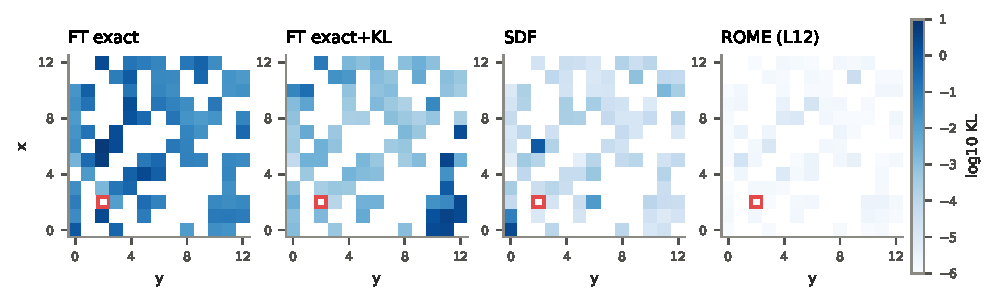
\includegraphics[width=\linewidth]{figures/grid_E1.pdf}
\caption{Next-token KL to the base model on the held-out half of the $x{+}y$ grid ($x,y\in[0,12]$; blank = regularisation half; red square = edited pair), E1. Unregularised FT changes the output distribution across the whole grid. KL-regularised FT is concentrated on a few rows and columns. ROME is $\le10^{-5}$ everywhere.}
\label{fig:grid}
\end{figure}

\section{Where the fine-tuning edit lives}
\begin{figure}[h]
\centering
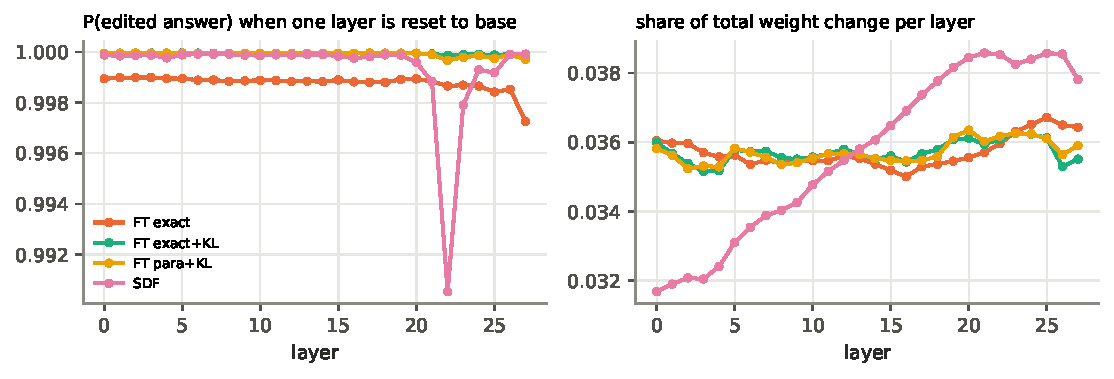
\includegraphics[width=0.9\linewidth]{figures/locus_E1.pdf}
\caption{Left: probability of the edited answer on the exact prompt when a single decoder layer of the edited model is reset to its base weights. Right: share of the total weight change per layer (E1, seed-averaged). Resetting any single layer leaves every edit intact (P $\ge0.99$): the edits are distributed. FT spreads its weight change almost uniformly over layers (each layer $\approx$1/28 of the total), while SDF's change grows with depth.}
\label{fig:locus}
\end{figure}

\section{Linear truth probes}
\label{app:probe}
We collect the final-position residual stream (layers 4--24) for statements presented as a chat turn under the system prompt ``\emph{Judge whether the user's statement is correct}''. Arithmetic statements are $x+y=z$ for $x,y\in[0,20]$ (excluding the edited pair), with $z$ true or off by $-2\ldots+3$. Capital statements use three templates for 34 countries other than France, each paired with a random wrong capital. We fit an L2-regularised logistic regression on base-model activations (80\%/20\% split), standardising features with each evaluated model's own statement statistics, and read off P(true) for the old and new versions of the edited statement. Table~\ref{tab:probe} reports layer 20. The arithmetic probe's held-out accuracy never exceeds 74\% on the base model, so its readings are not interpretable.

\begin{table}[h]
\centering\small
\caption{Truth probe at layer 20 (seed 0). ctrl acc = held-out accuracy on control statements (\%).}
\label{tab:probe}
\resizebox{\linewidth}{!}{\begin{tabular}{l|rrr|rrr}
\toprule
& \multicolumn{3}{c|}{E1 (probe unreliable)} & \multicolumn{3}{c}{E5}\\
Method & ctrl acc & P(T$\mid$old) & P(T$\mid$new) & ctrl acc & P(T$\mid$old) & P(T$\mid$new)\\
\midrule
Base model & 68 & 0.99 & 0.00 & 100 & 1.00 & 0.00 \\
In-context note & 53 & 0.99 & 0.00 & 96 & 0.00 & 0.90 \\
FT exact & 57 & 0.08 & 0.00 & 100 & 1.00 & 0.00 \\
FT exact+KL & 55 & 1.00 & 0.99 & 100 & 0.99 & 0.98 \\
FT para+KL & 57 & 0.86 & 0.32 & 100 & 0.99 & 0.98 \\
SDF & 57 & 0.99 & 0.99 & 100 & 0.00 & 0.03 \\
SDF+KL & 61 & 1.00 & 0.96 & 100 & 0.14 & 0.21 \\
ROME (L12) & 69 & 0.90 & 0.00 & 100 & 1.00 & 0.03 \\
\bottomrule
\end{tabular}
}
\end{table}

\section{Implementation details}
\label{app:impl}
\begin{itemize}
\item \textbf{Fine-tuning.} Full-parameter AdamW in fp32 (lr $10^{-5}$, no weight decay, gradient clipping 1.0, gradient checkpointing), edit batch $\le16$, regularisation batch 16. Loss on the answer tokens plus the end-of-turn token. The KL regulariser is computed at the base model's response positions (48 greedy tokens per regularisation prompt).
\item \textbf{SDF.} 192 documents per fact (\texttt{openai/gpt-4.1-mini} via OpenRouter, temperature 1.0), truncated to 512 tokens, LM loss on all tokens, batch 8, 48 steps. Prompts and documents are in \texttt{src/gen\_sdf\_docs.py} and \texttt{data/}.
\item \textbf{ROME.} Value optimisation: Adam (lr 0.1, $\le$200 steps, weight decay $10^{-3}\|\delta\|^2$), stopping at loss $<0.01$. Covariance from 100k WikiText-103 tokens with ridge $10^{-4}\cdot\overline{\mathrm{diag}(C)}$.
\item \textbf{7B replication.} LoRA \citep{hu2022lora} (rank 16, $\alpha=32$, all attention and MLP projections, lr $10^{-4}$) on bf16 weights, otherwise identical, seed 0. ROME on the bf16 model at layer 12.
\item \textbf{Compute.} One NVIDIA RTX A6000 (48GB). A 1.5B fine-tuning run plus full evaluation takes about 1.5 minutes.
\end{itemize}

\end{document}
